\documentclass[11pt]{article}

% ---------------------------------------------------------------------------
%  Preamble (pdflatex-safe)
% ---------------------------------------------------------------------------
\usepackage[a4paper,margin=1.7cm]{geometry}
\usepackage{amsmath,amssymb}
\usepackage{tikz}
\usepackage{tikz-cd}
\usetikzlibrary{arrows.meta,positioning,calc,fit,backgrounds,
  shapes.geometric,decorations.pathreplacing,decorations.markings,shadows}
\usepackage[most]{tcolorbox}
\usepackage{listings}
\usepackage{parskip}
\usepackage{xcolor}

\definecolor{ink}{RGB}{40,40,40}
\definecolor{soft}{RGB}{245,245,248}
% layer colours (bottom to top of the ladder)
\definecolor{cAb}{RGB}{30,90,160}     % Ab / preadditive
\definecolor{cMod}{RGB}{30,140,80}    % Mod_F2
\definecolor{cMon}{RGB}{200,120,0}    % monoid object
\definecolor{cDual}{RGB}{150,60,160}  % dualizable / finite
\definecolor{cField}{RGB}{190,50,60}  % the one division / field input
\definecolor{res}{RGB}{190,50,60}

% ----- Lean listing style (unicode via listings literate) -----
\definecolor{leanbg}{RGB}{248,248,252}
\definecolor{leankw}{RGB}{140,20,140}
\definecolor{leancm}{RGB}{110,120,130}
\lstdefinestyle{lean}{
  basicstyle=\ttfamily\footnotesize,
  backgroundcolor=\color{leanbg},
  frame=single, framesep=4pt, rulecolor=\color{gray!40},
  breaklines=true, columns=fullflexible, keepspaces=true,
  keywordstyle=\color{leankw}\bfseries,
  commentstyle=\color{leancm}\itshape,
  morecomment=[l]{--},
  morekeywords={theorem,lemma,def,by,namespace,end,variable,open,rw,exact,
    have,intro,induction,with,fun,Prop,Field,Fintype,CharP,set,apply,refine,
    rcases,cases,unfold,simp,ring,ring_nf,grind,linear_combination,omit,in,
    positivity,conv_lhs,show,from,where,noncomputable,Type,MonoidHom,instance,
    CommRing,NoZeroDivisors,Algebra,structure,End},
  literate=
    {∑}{{$\sum$}}1 {∈}{{$\in$}}1 {ℕ}{{$\mathbb{N}$}}1 {→}{{$\to$}}1
    {≠}{{$\neq$}}1 {∨}{{$\vee$}}1 {∧}{{$\wedge$}}1 {∀}{{$\forall$}}1
    {·}{{$\cdot$}}1 {ℓ}{{$\ell$}}1 {≡}{{$\equiv$}}1 {𝔽}{{$\mathbb{F}$}}1
    {⟹}{{$\Rightarrow$}}1 {⟨}{{$\langle$}}1 {⟩}{{$\rangle$}}1
    {≤}{{$\le$}}1 {↦}{{$\mapsto$}}1 {←}{{$\leftarrow$}}1 {×}{{$\times$}}1
    {σ}{{$\sigma$}}1 {φ}{{$\varphi$}}1 {Φ}{{$\Phi$}}1 {τ}{{$\tau$}}1
    {θ}{{$\theta$}}1 {μ}{{$\mu$}}1 {ν}{{$\nu$}}1 {ρ}{{$\rho$}}1
    {γ}{{$\gamma$}}1 {β}{{$\beta$}}1 {α}{{$\alpha$}}1 {κ}{{$\kappa$}}1
    {ε}{{$\varepsilon$}}1 {∘}{{$\circ$}}1 {⥤}{{$\rightsquigarrow$}}1
    {²}{{\textsuperscript{2}}}1 {ⁿ}{{\textsuperscript{n}}}1
    {ⁱ}{{\textsuperscript{i}}}1 {ʲ}{{\textsuperscript{j}}}1 {ᵏ}{{\textsuperscript{k}}}1
    {ʳ}{{\textsuperscript{r}}}1 {≃}{{$\simeq$}}1 {ₙ}{{$_n$}}1
    {→ₐ}{{$\to_{a}$}}1 {→+}{{$\to_{+}$}}1 {≃+}{{$\simeq_{+}$}}1 {→*}{{$\to^{*}$}}1
    {₀}{{$_0$}}1 {₁}{{$_1$}}1 {₂}{{$_2$}}1
    {@N}{{\ensuremath{\mathbb{N}}}}1 {@f}{{\ensuremath{\varphi}}}1
    {@e}{{\ensuremath{\varepsilon}}}1 {@s}{{\ensuremath{\sum}}}1
    {@m}{{\ensuremath{\in}}}1 {@q}{{\ensuremath{\neq}}}1
    {@F}{{\ensuremath{\mathbb{F}_2}}}1 {@L}{{\ensuremath{\leftarrow}}}1
    {@pn}{{\textsuperscript{n}}}1
}
\lstset{style=lean}

\newtcolorbox{note}[1][]{colback=soft,colframe=ink,boxrule=0.4pt,
  arc=2pt,left=6pt,right=6pt,top=4pt,bottom=4pt,#1}

\tikzset{
  obj/.style={draw=ink,rounded corners=3pt,fill=soft,inner sep=5pt,
    font=\small,align=center},
  ar/.style={-{Stealth[length=2.2mm]},shorten >=1pt,shorten <=1pt},
  tag/.style={font=\footnotesize\itshape,inner sep=1pt},
  rung/.style={draw,rounded corners=3pt,align=center,inner sep=6pt,
    font=\small,drop shadow={opacity=.15}},
}
\newcommand{\lc}[1]{\texttt{\small #1}}
\newcommand{\Tr}{\operatorname{Tr}}
\newcommand{\Nn}{\mathbb{N}}
\newcommand{\Ff}{\mathbb{F}_2}
\newcommand{\Fq}{\mathbb{F}_{2^{n}}}
\newcommand{\End}{\operatorname{End}}
\newcommand{\Module}{\operatorname{Module}}
\newcommand{\CharP}{\operatorname{CharP}}
\newcommand{\Algebra}{\operatorname{Algebra}}

\title{\bfseries The Algebra and Category Layers of the\\
  Dobbertin $(1)\!\Rightarrow\!(2)$ Formalisation\\[4pt]
  \large A visual field-guide to \lc{AlgebraLayer}, \lc{CategoryTheory},
  \lc{Categorical}, \lc{ObjectFirst}}
\author{}
\date{}

\begin{document}
\maketitle

\vspace{-1.2em}
\begin{note}\small
\textbf{One picture.} The whole first step of Dobbertin's Theorem~1 is one
endomorphism $\varphi$ (Frobenius, $x\mapsto x^{2}$) of one object, and one
identity, the telescope $(\varphi-1)\!\cdot\!\sum\varphi^{i}=\varphi^{\ell}-1$.
This note draws \emph{where each hypothesis lives}: the algebra layer strips the
carrier down to a bare commutative ring of characteristic~$2$ and isolates the
\emph{single} spot that needs a field; the category layer builds $\varphi$ and the
telescope up an \emph{enrichment ladder} in which every rung deletes one input by
absorbing it into the ambient object.
\end{note}

% ===========================================================================
\section{The two axes}

\begin{center}
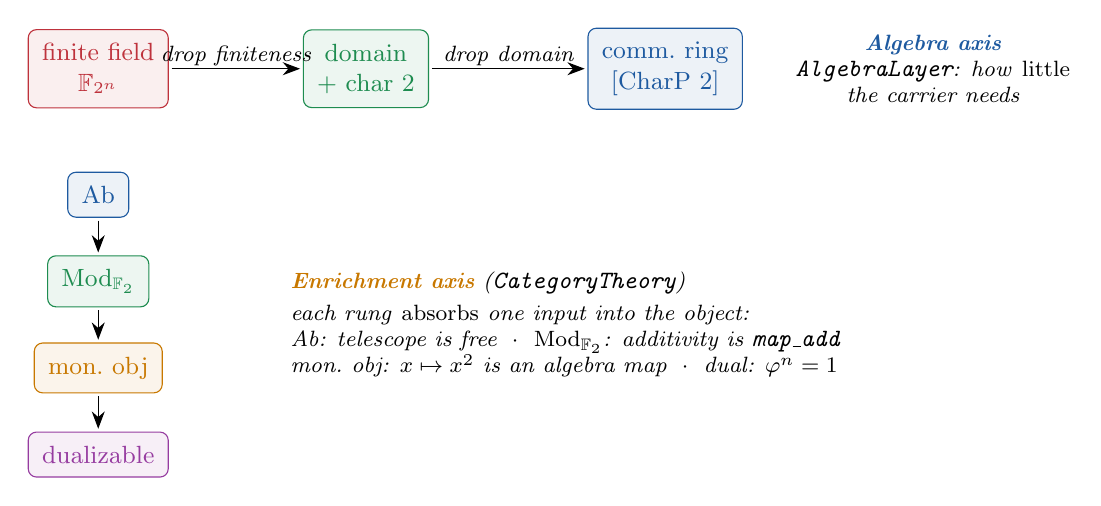
\begin{tikzpicture}[every node/.style={font=\footnotesize}]
  % horizontal: algebra generality axis
  \node[obj,cField,draw=cField,fill=cField!8] (fld) at (0,0) {finite field\\$\Fq$};
  \node[obj,cMod,draw=cMod,fill=cMod!8] (dom) at (3.4,0) {domain\\$+$ char $2$};
  \node[obj,cAb,draw=cAb,fill=cAb!8] (ring) at (7.2,0) {comm.\ ring\\ $[\text{CharP }2]$};
  \draw[ar] (fld) -- node[tag,above]{drop finiteness} (dom);
  \draw[ar] (dom) -- node[tag,above]{drop domain} (ring);
  \node[tag,align=center] at (10.6,0)
     {\textcolor{cAb}{\textbf{Algebra axis}}\\ \lc{AlgebraLayer}: how \emph{little}\\ the carrier needs};

  % vertical: enrichment ladder axis
  \node[obj,cAb,draw=cAb,fill=cAb!8]  (ab)  at (0,-1.6) {Ab};
  \node[obj,cMod,draw=cMod,fill=cMod!8] (mod) at (0,-2.7) {$\mathrm{Mod}_{\Ff}$};
  \node[obj,cMon,draw=cMon,fill=cMon!8] (mon) at (0,-3.8) {mon.\ obj};
  \node[obj,cDual,draw=cDual,fill=cDual!8] (du) at (0,-4.9) {dualizable};
  \draw[ar] (ab) -- (mod); \draw[ar] (mod) -- (mon); \draw[ar] (mon) -- (du);
  \node[tag,align=left,anchor=west] at (2.4,-3.25)
     {\textcolor{cMon}{\textbf{Enrichment axis}} (\lc{CategoryTheory})\\[2pt]
      each rung \emph{absorbs} one input into the object:\\
      Ab: telescope is free \;$\cdot$\; $\mathrm{Mod}_{\Ff}$: additivity is \lc{map\_add}\\
      mon.\ obj: $x\mapsto x^{2}$ is an algebra map \;$\cdot$\; dual: $\varphi^{n}=1$};
\end{tikzpicture}
\end{center}

\begin{center}\small
\renewcommand{\arraystretch}{1.3}
\begin{tabular}{@{}p{3.0cm}p{6.1cm}p{4.9cm}@{}}
\hline
\textbf{module} & \textbf{what it shows} & \textbf{headline}\\
\hline
\lc{AlgebraLayer} & the trace/telescope layer over \emph{any} comm.\ ring of char $2$; field used once & \lc{alg\_equation2\_of\_equation1}\\
\lc{CategoryTheory} & $\varphi$ and telescope up the enrichment ladder & \lc{equation2\_of\_equation1\_cat}\\
\lc{Categorical} & the four abstract patterns behind the bricks & (structure, not proof)\\
\lc{ObjectFirst} & the type-class bundle collapsed into the object & \lc{equation2\_of\_equation1\_obj}\\
\hline
\end{tabular}
\end{center}

% ===========================================================================
\section{Algebra layer: how little the carrier needs}

The entire telescope layer is proved with \lc{[CommRing R] [CharP R 2]} only.
Field-ness enters at exactly \emph{one} arrow --- the division by $x^{2^{k}}$.

\begin{center}
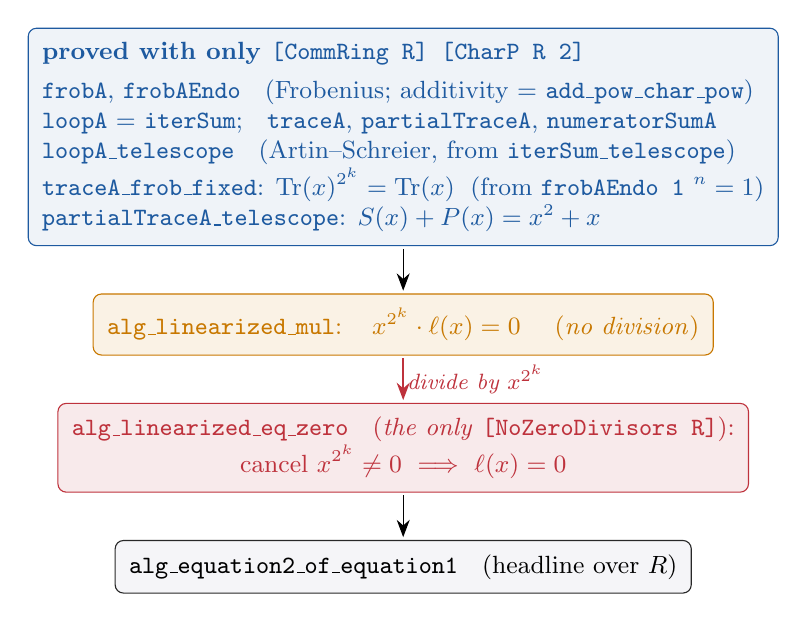
\begin{tikzpicture}[every node/.style={font=\footnotesize},node distance=6mm]
  \node[obj,cAb,draw=cAb,fill=cAb!7,align=left] (top)
    {\textbf{\textcolor{cAb}{proved with only \lc{[CommRing R] [CharP R 2]}}}\\[3pt]
     \lc{frobA}, \lc{frobAEndo} \; (Frobenius; additivity $=$ \lc{add\_pow\_char\_pow})\\
     \lc{loopA} $=$ \lc{iterSum}; \; \lc{traceA}, \lc{partialTraceA}, \lc{numeratorSumA}\\
     \lc{loopA\_telescope} \; (Artin--Schreier, from \lc{iterSum\_telescope})\\
     \lc{traceA\_frob\_fixed}: $\Tr(x)^{2^{k}}=\Tr(x)$ \;(from \lc{frobAEndo 1} $^{n}=1$)\\
     \lc{partialTraceA\_telescope}: $S(x)+P(x)=x^{2}+x$};
  \node[obj,cMon,draw=cMon,fill=cMon!10,below=of top,align=center]
    (mul) {\lc{alg\_linearized\_mul}: \; $x^{2^{k}}\cdot \ell(x)=0$ \quad(\emph{no division})};
  \node[obj,cField,draw=cField,fill=cField!10,below=of mul,align=center]
    (div) {\textbf{\textcolor{cField}{\lc{alg\_linearized\_eq\_zero}}} \; (\emph{the only} \lc{[NoZeroDivisors R]}):
      \\ cancel $x^{2^{k}}\neq0$ \;$\Longrightarrow$\; $\ell(x)=0$};
  \node[obj,draw=ink,below=of div,align=center]
    (hd) {\lc{alg\_equation2\_of\_equation1} \; (headline over $R$)};
  \draw[ar] (top) -- (mul);
  \draw[ar,cField,thick] (mul) -- node[tag,right]{\textcolor{cField}{divide by $x^{2^{k}}$}} (div);
  \draw[ar] (div) -- (hd);
\end{tikzpicture}
\end{center}

\begin{lstlisting}
variable {R : Type*} [CommRing R] [CharP R 2]           -- @F-algebra, nothing more

lemma alg_linearized_mul (k : @N) {c x @e S P : R}       -- NO field, NO division
    (hS : S = P ^ (2 ^ k)) (hSP : S + P = x ^ 2 + x)
    (h@efix : @e ^ (2 ^ k) = @e) (hsol : S + @e = c * x ^ (2 ^ k + 1)) :
    x ^ (2 ^ k) * (c ^ (2 ^ k) * x ^ (2 ^ (2 * k)) + x ^ (2 ^ k) + c * x + 1) = 0

lemma alg_linearized_eq_zero [NoZeroDivisors R] ... (hx : x @q 0) :  -- @L field enters here, once
    c ^ (2 ^ k) * x ^ (2 ^ (2 * k)) + x ^ (2 ^ k) + c * x + 1 = 0
\end{lstlisting}

\begin{note}
\textbf{Why no field above the red line.} $\Tr(x)^{2^{k}}=\Tr(x)$ is
\lc{traceA\_frob\_fixed}, a corollary of the telescope with $\varphi^{n}=1$; it
supplies $\varepsilon^{2^{k}}=\varepsilon$ for $\varepsilon=\alpha\,\Tr(x)$
\emph{without} needing $\Tr(x)\in\{0,1\}$. So the field-only fact ``the trace is a
bit'' is never used in the linearization --- the only field step is the final
cancellation.
\end{note}

\subsection*{The field is one instance}

\begin{center}
\begin{tikzcd}[column sep=large,row sep=small]
\text{\lc{alg\_equation2\_of\_equation1}} \arrow[d,swap,"{\text{set }R=\Fq}"]
  & {[\text{CommRing }R]\,[\text{CharP }R\,2]\,[\text{NoZeroDivisors }R]} \\
\text{\lc{equation2\_of\_equation1\_of\_finField}}
  & \Fq:\ \text{Fermat }=\ \text{\lc{frobAEndo\_pow\_card\_field}}\ \Rightarrow\ \varphi^{n}=1
\end{tikzcd}
\end{center}
The finite field is recovered as the \lc{IsDomain} specialization: Fermat
discharges $\varphi^{n}=1$ and field-ness discharges the one division.

% ===========================================================================
\section{Category layer: the enrichment ladder}

Read the carrier not as a set but as an \emph{object} of a progressively richer
category. Each rung to the right makes one hand-proved input \emph{free}.

\begin{center}
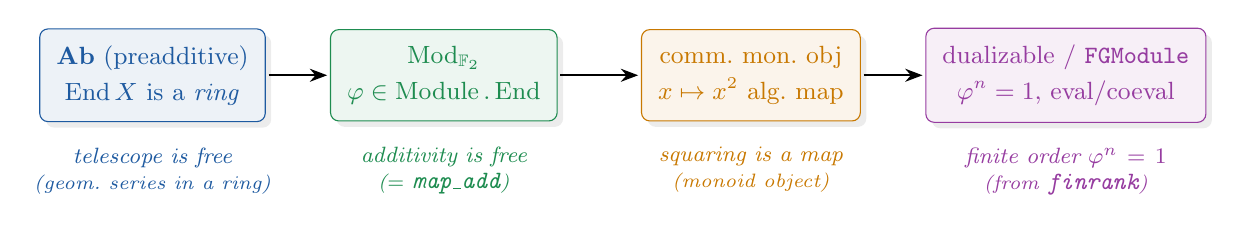
\begin{tikzpicture}[every node/.style={font=\footnotesize}]
  \node[rung,cAb,draw=cAb,fill=cAb!8]   (ab)  at (0,0)
     {\textbf{Ab} (preadditive)\\[2pt]$\End X$ is a \emph{ring}};
  \node[rung,cMod,draw=cMod,fill=cMod!8] (mod) at (3.7,0)
     {$\mathrm{Mod}_{\Ff}$\\[2pt]$\varphi\in\Module.\End$};
  \node[rung,cMon,draw=cMon,fill=cMon!8] (mon) at (7.6,0)
     {comm.\ mon.\ obj\\[2pt]$x\mapsto x^{2}$ alg.\ map};
  \node[rung,cDual,draw=cDual,fill=cDual!8] (du) at (11.6,0)
     {dualizable / \lc{FGModule}\\[2pt]$\varphi^{n}=1$, eval/coeval};
  \draw[ar,thick] (ab)  -- (mod);
  \draw[ar,thick] (mod) -- (mon);
  \draw[ar,thick] (mon) -- (du);
  % what each rung buys
  \node[tag,cAb,align=center,text width=3.1cm,below=8pt of ab]
     {telescope is free\\ {\scriptsize(geom.\ series in a ring)}};
  \node[tag,cMod,align=center,text width=3.1cm,below=8pt of mod]
     {additivity is free\\ {\scriptsize($=$ \lc{map\_add})}};
  \node[tag,cMon,align=center,text width=3.1cm,below=8pt of mon]
     {squaring is a map\\ {\scriptsize(monoid object)}};
  \node[tag,cDual,align=center,text width=3.1cm,below=8pt of du]
     {finite order $\varphi^{n}=1$\\ {\scriptsize(from \lc{finrank})}};
\end{tikzpicture}
\end{center}

\paragraph{Rung 1 --- Ab.} In the endomorphism \emph{ring} of any object of a
preadditive category, the telescope is the geometric series --- no field, no
characteristic, no finiteness:
\begin{lstlisting}
theorem preadditive_telescope (@f : End X) (len : @N) :
    (@f - 1) * (@s i @m range len, @f ^ i) = @f ^ len - 1 := mul_geom_sum @f len
\end{lstlisting}

\paragraph{Rung 2 --- $\mathrm{Mod}_{\Ff}$, and the ring isomorphism.} Over the
base object $\Ff=\lc{ZMod 2}$ the Frobenius is a \emph{morphism of modules}
$\varphi=\lc{frobLin}$, so its additivity is \lc{map\_add}. The ring it lives in
\emph{is} the object's categorical $\End$:
\begin{center}
\begin{tikzcd}[column sep=huge,row sep=tiny]
\End(\lc{ModuleCat.of }\Ff\ F) \arrow[r,"{\lc{endRingEquiv}}","\simeq_{+*}"'] & \Module.\End\ \Ff\ F\\
\lc{frobMor} \arrow[r,mapsto] & \lc{frobLin}
\end{tikzcd}
\end{center}
so \lc{frobMor\_telescope} (run as arrow data) transports to \lc{frobLin\_telescope}.

\paragraph{Rung 3 --- commutative monoid object.} A commutative monoid object of
$(\lc{ModuleCat }\Ff,\otimes)$ \emph{is} a $\Ff$-algebra
(\lc{MonModuleEquivalenceAlgebra}); this is \emph{why} $x\mapsto x^{2}$ is an
algebra map, hence why \lc{frobLin} exists at all.

\paragraph{Rung 4 --- dualizable / finite.} A finite field is a
finite-dimensional, hence \emph{dualizable}, object of \lc{FGModuleCat} $\Ff$.
Its finite \emph{dimension} --- not raw cardinality --- forces $\varphi^{n}=1$.
The annihilating polynomial $X^{n}-1$ is read off through a \emph{monoid map}:
\begin{center}
\begin{tikzcd}[column sep=huge,row sep=large]
(F \to_{a}[\Ff] F) \arrow[r,"{\lc{algEndToLin}}","\to^{*}"'] \arrow[d,swap,"{\operatorname{ord}=\lc{finrank}}"]
  & \Module.\End\ \Ff\ F \arrow[d,"{(-)^{n}}"]\\
\lc{frobeniusAlgHom} \arrow[r,mapsto] \arrow[loop left,"{\operatorname{ord}=[F:\Ff]}"']
  & \lc{frobLin},\quad \lc{frobLin}^{n}=1
\end{tikzcd}
\end{center}
\begin{lstlisting}
lemma frobLin_orderOf : orderOf (frobeniusAlgHom (ZMod 2) F) = Module.finrank (ZMod 2) F
lemma frobLin_pow_finrank : (frobLin (F := F)) ^ (Module.finrank (ZMod 2) F) = 1
   := by rw [@L algEndToLin_frobeniusAlgHom, @L map_pow, @L frobLin_orderOf,
             pow_orderOf_eq_one, map_one]        -- @f@pn = 1 from finite dimension
\end{lstlisting}

% ===========================================================================
\section{Reassembly: the telescope drives the two facts}

Both facts the paper uses are the \emph{one} telescope, applied to $\varphi$ (at
length $n$) and to $\varphi^{k}$ (at length $k'$).

\begin{center}
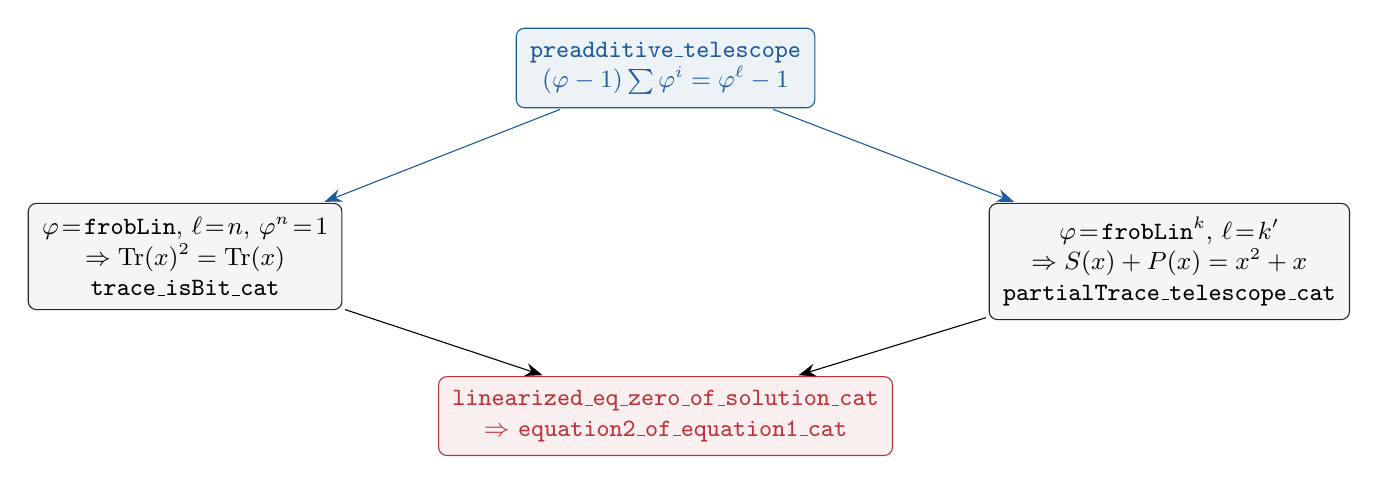
\begin{tikzpicture}[every node/.style={font=\footnotesize},node distance=5mm]
  \node[obj,cAb,draw=cAb,fill=cAb!8,align=center] (tel)
    {\lc{preadditive\_telescope}\\ $(\varphi-1)\sum\varphi^{i}=\varphi^{\ell}-1$};
  \node[obj,below left=12mm and 22mm of tel,align=center] (bit)
    {$\varphi\!=\!\lc{frobLin}$, $\ell\!=\!n$, $\varphi^{n}\!=\!1$\\
     $\Rightarrow \Tr(x)^{2}=\Tr(x)$\\ \textbf{\lc{trace\_isBit\_cat}}};
  \node[obj,below right=12mm and 22mm of tel,align=center] (asc)
    {$\varphi\!=\!\lc{frobLin}^{k}$, $\ell\!=\!k'$\\
     $\Rightarrow S(x)+P(x)=x^{2}+x$\\ \textbf{\lc{partialTrace\_telescope\_cat}}};
  \node[obj,cField,draw=cField,fill=cField!8,below=34mm of tel,align=center] (hd)
    {\lc{linearized\_eq\_zero\_of\_solution\_cat}\\ $\Rightarrow$ \textbf{\lc{equation2\_of\_equation1\_cat}}};
  \draw[ar,cAb] (tel) -- (bit);
  \draw[ar,cAb] (tel) -- (asc);
  \draw[ar] (bit) -- (hd);
  \draw[ar] (asc) -- (hd);
\end{tikzpicture}
\end{center}

% ===========================================================================
\section{Object-first: collapse the type-class bundle}

The concrete proof carries \lc{[Field F] [Fintype F] [CharP F 2]} as three
inputs. Reading $F$ as an \emph{object} of $\mathrm{Mod}_{\Ff}$ makes char~$2$ a
\emph{consequence}: the structure map $\Ff\hookrightarrow F$ is injective.

\begin{center}
\begin{tikzcd}[column sep={4.4cm,between origins},row sep=small]
{[\Algebra\ (\lc{ZMod 2})\ F]} \arrow[r,"{\lc{algebraMap}\text{ inj.}}"]
  & \Ff\hookrightarrow F \arrow[r,"{\lc{charP\_of\_inj\_algMap}}"]
  & {[\CharP\ F\ 2]}
\end{tikzcd}
\ (\text{derived instance }\lc{objCharP})
\end{center}
\begin{lstlisting}
variable {F : Type} [Field F] [Fintype F] [Algebra (ZMod 2) F]  -- the object
instance objCharP : CharP F 2 :=                                 -- no longer a hypothesis
  charP_of_injective_algebraMap (algebraMap (ZMod 2) F).injective 2

theorem equation2_of_equation1_obj ...   -- headline with the collapsed bundle
\end{lstlisting}
Multiplication itself comes from the monoid object
(\lc{objMonObj}, \lc{objAlg}), and the whole categorical chain
(\lc{objFrobLin\_telescope}, \lc{objFrobLin\_pow\_finrank}, \lc{objTrace\_isBit})
runs uniformly in universe $0$.

% ===========================================================================
\section{The whole picture}

\begin{center}
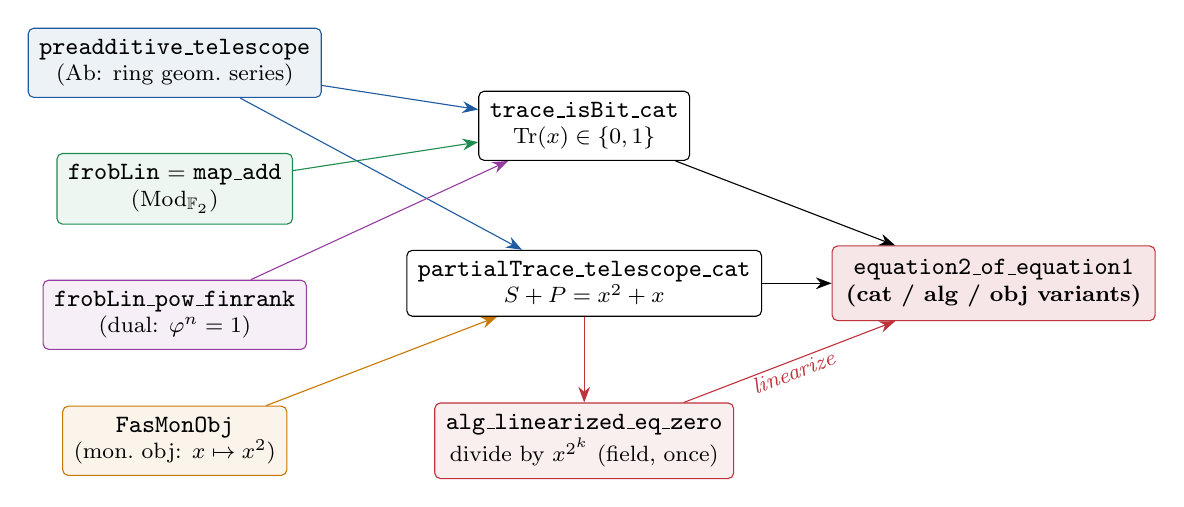
\begin{tikzpicture}[
  every node/.style={font=\footnotesize},
  box/.style={draw,rounded corners=2pt,align=center,inner sep=4pt},
  hd/.style ={draw,rounded corners=2pt,align=center,inner sep=5pt,
              fill=res!12,draw=res,font=\footnotesize\bfseries},
  fl/.style={-{Stealth[length=2mm]}}]
  % abstract inputs (left)
  \node[box,draw=cAb,fill=cAb!8]  (tel) at (0,2.2)  {\lc{preadditive\_telescope}\\(Ab: ring geom.\ series)};
  \node[box,draw=cMod,fill=cMod!8](fro) at (0,0.6)  {\lc{frobLin} $=$ \lc{map\_add}\\($\mathrm{Mod}_{\Ff}$)};
  \node[box,draw=cDual,fill=cDual!8](ord) at (0,-1.0){\lc{frobLin\_pow\_finrank}\\(dual: $\varphi^{n}=1$)};
  \node[box,draw=cMon,fill=cMon!8](mon) at (0,-2.6) {\lc{FasMonObj}\\(mon.\ obj: $x\mapsto x^{2}$)};
  % middle: the two facts
  \node[box] (bit) at (5.2,1.4) {\lc{trace\_isBit\_cat}\\ $\Tr(x)\in\{0,1\}$};
  \node[box] (asc) at (5.2,-0.6){\lc{partialTrace\_telescope\_cat}\\ $S+P=x^{2}+x$};
  % algebra-layer division
  \node[box,draw=cField,fill=cField!8] (div) at (5.2,-2.6)
     {\lc{alg\_linearized\_eq\_zero}\\ divide by $x^{2^{k}}$ (field, once)};
  % headline (right)
  \node[hd] (head) at (10.4,-0.6) {\lc{equation2\_of\_equation1}\\(cat / alg / obj variants)};
  \draw[fl,cAb]  (tel) -- (bit);
  \draw[fl,cAb]  (tel) -- (asc);
  \draw[fl,cMod] (fro) -- (bit);
  \draw[fl,cDual](ord) -- (bit);
  \draw[fl,cMon] (mon) -- (asc);
  \draw[fl] (bit) -- (head);
  \draw[fl] (asc) -- (head);
  \draw[fl,cField] (div) -- node[tag,below,sloped]{linearize} (head);
  \draw[fl,cField] (asc) -- (div);
\end{tikzpicture}
\end{center}

\begin{note}
\textbf{Soundness.} \lc{AlgebraLayer}, \lc{CategoryTheory}, \lc{Categorical} and
\lc{ObjectFirst} build \lc{sorry}-free; the headlines
(\lc{alg\_equation2\_of\_equation1}, \lc{equation2\_of\_equation1\_cat},
\lc{equation2\_of\_equation1\_obj}, \lc{equation2\_of\_equation1\_of\_finField})
depend only on \lc{propext}, \lc{Classical.choice}, \lc{Quot.sound}. The category
layer supplies the \emph{shape}; the algebra layer pins the \emph{one} place a
field is needed.
\end{note}

\end{document}
